\documentclass{article}
\usepackage{a4}
\usepackage[latin1]{inputenc}
\usepackage{verbatim}
\usepackage{hyperref}
\usepackage{graphicx}
\usepackage{longtable}


%\input{udmath}


\hypersetup{bookmarks, bookmarksopen,
  pdftitle={VYM - Una herramiento para pensamiento visual },
  pdfauthor={Uwe Drechsel},    
  pdfsubject={map},
  pdfkeywords={map, tool},
  pdfpagemode={UseOutlines},                                 
  bookmarksopenlevel={1},   
  colorlinks={true},     
  linkcolor={blue},
  urlcolor={green},
  citecolor={red}} 


\newcommand{\vym}{{\sc vym }}
\newcommand{\ra}{$\longrightarrow$}
\newcommand{\la}{$\longleftarrow$}
\newcommand{\ua}{$\uparrow$}
\newcommand{\da}{$\downarrow$}
\newcommand{\key}[1]{[#1]}

\begin{document}
\title{
    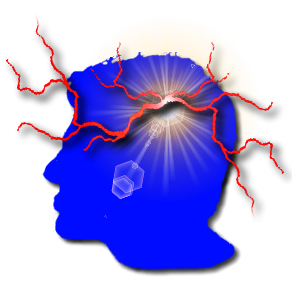
\includegraphics[width=8cm]{images/vym-logo-new.png}
    \\
VYM \\ -- \\View Your Mind\\ {\small Versi\'on 1.8.0}}
\author{\textcopyright Uwe Drechsel  }


\maketitle

\newpage

\tableofcontents

\newpage
\section{Creditos}
\subsection{Autor}
Uwe Drechsel
\subsection{Traducci\'on}
Traducci\'on a cargo del proyecto ACLibre (Academia y Conocimiento Libre)

P\'agina web: 
        \href{http://ieee.udistrital.edu.co/aclibre}{http://ieee.udistrital.edu.co/aclibre}

Correo: 
        \href{mailto:aclibre@gmail.com}{aclibre@gmail.com}
\subsection{Participantes}
\begin{center}
\begin{tabular}{|p{7cm}|p{5.5cm}|} \hline
    Encargado & Actividad \\ \hline
    \begin{itemize}
       \item Vanessa Carolina Guti\'errez Sanchez
       \item Erika Tatiana Luque Melo
       \item Jeffrey Steve Borb\'on Sanabria
       \item John Edisson Ortiz Rom\'an
    \end{itemize} &
    \begin{itemize}
        \item Traducci\'onl
        \item Revisi\'on y correcciones varias
        \item Estructuraci\'on y exporte
        \item Revisi\'on y correcciones varias
    \end{itemize}     \\ \hline
\end{tabular}   
\end{center}

\section{Introducci\'on}
\subsection{?`Qu\'e es un mapa \vym?}
Un mapa \vym (en pocas palabras mapa) es una estructura con forma de \'arbol:
\begin{center}
    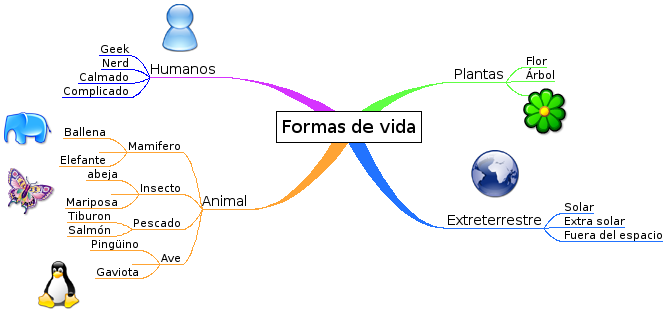
\includegraphics[width=12cm]{images/example1_es.png}
\end{center}
Estos mapas pueden ser dibujados a mano o en un portafolio y ayudan a estructurar ideas. Mientras que una estructura en forma de \'arbol, como las de arriba, puede ser dibujada a mano, \vym ofrece gran variedad de opciones para trabajar con estos mapas. \vym no es otro software de dibujo, sino una herramienta para guardar y modificar informaci\'on de una manera intuitiva. Por ejemplo, puede reordenar partes del mapa con solo presionar una tecla o agregar informaci\'on, como un correo electr\'onico completo, con solo hacer un click.

Una vez que ha finalizado en recoger y organizar sus ideas, puede f\'acilmente generar por ejemplo, una presentaci\'on en OpenOffice basada en un mapa.

\subsection{?`Por qu\'e debo usar mapas? Tiempo, Espacio y su Cerebro?}
\subsubsection*{Espacio}
Un mapa puede concentrar contenido muy complejo en un espacio peque\~no como por ejemplo un pedazo de papel. Los mapas ayudan a utilizar los dos lados del cerebro: tanto el l\'ogico como el creativo (mediante el uso de im\'agenes, colores y palabras claves en el mapa). Esta es una t\'ecnica para organizar la manera en que piensa: Puede ayudarlo a trav\'es del desarrollo, clasificaci\'on y memorizaci\'on de sus ideas.

\subsubsection*{Tiempo}
Como solo utiliza palabras claves y dibujos, es mucho mas r\'apido que las tradicionales notas. Su cerebro memoriza las cosas asoci\'andolas con otras - un mapa hace uso de esas conexiones y estimula nuevas asociaciones.


\subsubsection*{Su Cerebro}
En 1960 el Prof. Roger Sperry descubri\'o que los hemisferios del cerebro humano realizan diferentes tareas (por supuesto que ambos pueden realizar b\'asicamente lo mismo):
\begin{center}
\begin{tabular}{|p{5.5cm}|p{5.5cm}|} \hline
    Lado izquierdo & Lado derecho \\ \hline
    \begin{itemize}
       \item Dialogo y Escritura
       \item N\'umeros
       \item Razonamiento L\'ogico
       \item An\'alisis y Detalles
       \item Ciencia
       \item Razonamiento Lineal
       \item Concepto del Tiempo
    \end{itemize} &
    \begin{itemize}
        \item Lenguaje Corporal
        \item Razonamiento visual, so\~nar despierto.
        \item Intuici\'on y Emociones.
        \item Perspectiva de las cosas.
        \item Creatividad
        \item Arte, M\'usica, Baile
        \item Razonamiento no-lineal, conectando cosas
        \item Ubicaci\'on en el espacio
    \end{itemize}     \\ \hline
\end{tabular}   
\end{center}
En nuestra sociedad orientada a la ciencia hemos aprendido a depender principalmente del lado izquierdo del cerebro, del "racional". En otras culturas, especialmente los nativo americanos y otras culturas antiguas, el lado derecho es mucho mas importante. Los mapas son solo una forma de estimular ese otro lado y hacer uso de los recursos adicionales que todos tenemos.


\subsection{?`D\'onde puedo utilizar un mapa?}
Aqu\'i hay algunos ejemplos de como puede utilizar los mapas:
\begin{itemize}
    \item Para preparar art\'iculos, ensayos, libros, charlas, \ldots
    \item Para organizar informaci\'on compleja
    \item Para memorizar hechos, personas, vocabulario, \ldots
    \item Para ordenar correos electr\'onicos, archivos y marcadores en su computador
    \item Para moderar conferencias.
\end{itemize}

\subsection{Que no debe hacer con un mapa...}
Un mapa dibujado por alguien muestra la forma en que su autor piensa. No existe lo correcto o incorrecto en la forma en que es dibujado, as\'i que no existe forma de criticarlo. "Es, lo que es" ({\sc F.~Lehmann}).

\subsection{Recursos de Internet} 
Un buen punto de partida para conocer mas acerca de los mapas en general es la Wikipedia:
\begin{itemize}
    \item Ingl\'es: 
        \href{http://en.wikipedia.org/wiki/Mind_map}{http://en.wikipedia.org/wiki/Mind\_map}
    \item Alem\'an: 
        \href{http://de.wikipedia.org/wiki/Mindmap}{http://de.wikipedia.org/wiki/Mindmap}
\end{itemize}




\section{Concepto de \vym}
\subsection{Ventanas: Editor de mapas (mapeditor) y Editor de notas (noteeditor)}
\vym utiliza 2 ventanas: Un editor para el mapa y otro para las notas que son parte del mapa. Las llamaremos  {\em mapeditor} y {\em noteeditor}: 
\begin{center}
    \includegraphics[width=8cm]{images/windows_es.png}
\end{center}
Usualmente trabajara en el {\em Editor de mapas} para agregar, mover y reordenar las ramas. Las diferentes maneras de realizar esto se explicaran en \ref{mapeditor}. Puede guardar informaci\'on adicional en una {\em rama}, por ejemplo el contenido de un correo electr\'onico: Simplemente escriba o copie y pegue el correo en el {\em Editor de notas}. El trabajo con notas es explicado en \ref{noteeditor}.

\subsection{Barras del Men\'u y Men\'u desplegables}
En el tope de cada ventana encontrar\'a una barra de men\'u. Las opciones que all\'i se encuentran son similares a aquellas de otras aplicaciones. Note que muchas de la opciones (e incluso muchas m\'as) est\'an disponibles en los men\'u desplegables. Los cuales aparecen si hace un click derecho sobre un objeto en el mapa (en Mac OS X Comando-Click).

\subsection{Barra de Herramientas}
La barra de herramientas en la ventana principal ofrece r\'apido acceso a muchas funciones y adem\'as permite visualizar el estado de un objeto. Por ejemplo una parte del mapa puede ser ocultada cuando el mapa se exporta a una presentaci\'on de Open Office. Para indicar esto en el mapa, la rama tendr\'a un peque\~no s\'imbolo en forma de nube, el cual tambi\'en puede ser activado en la barra de herramientas.

Observe que puede reposicionar todas las barras de herramientas con solo arrastrarla. Por ejemplo puede mover la barra de herramientas con las banderas desde su posici\'on horizontal en la parte de arriba del Editor de mapas hasta una posici\'on vertical al lado derecho de la ventana. Incluso puede extraerlas y separarlas de las ventanas. O insertarla de nuevo en su posici\'on original.

\subsection{Mapas}
El mapa siempre tiene un {\em centro}. Este centro posee ramas como el tronco de un \'arbol. Cada {\em rama} a su vez albergar\'a otras {\em ramas}.
\begin{center}
    \includegraphics[width=10cm]{images/branches_es.png}
\end{center}
Llamaremos a las ramas conectadas directamente al centro del mapa {\em
ramas principales}, ya que determinan la posici\'on de sus ramas hijas.

El centro del mapa y todas las ramas tienen un {\em encabezado}. Este texto es el que se ve en el Editor de mapas. Por lo general debe ser una o pocas palabras, para tener un seguimiento mas sencillo del mapa.


En la barra de herramientas sobre el editor de mapas pueden verse varios s\'imbolos.
\begin{center}
    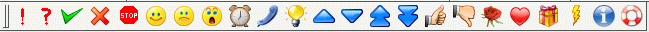
\includegraphics[width=8cm]{images/default-flags.png}
\end{center}
Estos son llamados {\em banderas} y pueden ser utilizadas para marcar en las ramas del mapa, por ejemplo, si algo es importante o cuestionable. Tambi\'en hay mas banderas configuradas autom\'aticamente por el \vym para mostrar informaci\'on adicional, por ejemplo cuando a existe para una rama en particular.

Por defecto algunas de estas banderas est\'an configuradas exclusivamente, por ejemplo cuando el pulgar hacia arriba esta seleccionado el pulgar hacia abajo no lo esta y vice versa. Puede modificar esta conducta por defecto en el men\' u de configuraciones.

\section{Editor de Mapas} \label {mapeditor}
\subsection{Abrir un mapa nuevo}
Luego de iniciar el \vym, 2 ventanas se abrir\'an: el Editor de mapas y el Editor de notas. Por lo general trabajara en ambas ventanas, pero por los momentos nos detendremos en el Editor de mapas.

Seleccione el centro del mapa "Nuevo mapa" en el medio del editor haciendo click izquierdo con el rat\'on. Cambiara a amarillo para mostrar que ha sido seleccionado. Existen varias formas de agregar una nueva rama al centro:
\begin{itemize}
    \item Utilizando el rat\'on: Abra el men\'u desplegable haciendo click con el bot\'on derecho del rat\'on (CTRL-Click en Mac) sobre el centro del mapa y escoge la opci\'on Adicionar \ra Agregar rama como hija. 
    \item Presione \key{Ins} o \key{A}
\end{itemize}
Una rama nueva aparecer\'a y podr\'a escribir el encabezado de esa rama. Para finalizar presione \key{Enter}.

A veces es \'util agregar una rama por encima o debajo de la actual, para ello utilice \key{Ins} junto a \key{Shift} o \key{Ctrl}. Tambi\'en es posible agregar una rama de manera que la selecci\'on actual se convierta en hija de la nueva rama, que seria como insertarla {\em antes} de lo seleccionado. Esto puede realizarse utilizando el men\'u desplegable.

\subsection{Navegando a trav\'es del mapa}
\subsubsection*{Seleccionar ramas}

Para seleccionar las ramas puede utilizar el bot\'on izquierdo del rat\'on o las teclas con flechas. Dependiendo de la {\em orientaci\'on} de la rama pulse \key{\la} o \key{\ra} para acercarse o alejarse del centro del mapa. Dentro de un grupo de ramas, que reciben el nombre de sub-\'arbol, puede utilizar \key{\ua} o \key{\da} para ir hacia arriba o abajo. Tambi\'en puede utilizar \key{Pos1} y \key{End} para seleccionar la primera o la ultima rama.

\subsubsection*{Zoom}
Mientras agrega mas y mas ramas el mapa podr\'ia superar en tama\~no a la ventana del Editor de mapas. Puede utilizar las barras de desplazamiento a la derecha y en la parte de abajo de la ventana del Editor para arrastrarlo, pero es mas f\'acil hacerlo utilizando el bot\'on izquierdo del rat\'on: Haga click sobre el espacio en blanco entre las ramas. El puntero del rat\'on cambiara su forma de flecha al de una mano, ahora mueva la parte visible del mapa para mostrar la parte deseada.

Si selecciona las ramas utilizando las flechas en el teclado, el mapa se arrastrara asegur\'andose de que la rama seleccionada este siempre visible.

Para trabajar con mapas muy grandes, la funci\'on del {\em zoom} es muy \'util. Puede usar:

\begin{itemize}
    \item Desde el men\'u Vista \ra Acercar
    \item Los botones de la barra de herramientas 
        \begin{center}
            \includegraphics[width=3cm]{images/zoom-buttons.png}
        \end{center}    
\end{itemize}   

La lupa con la cruz devuelve el zoom a su tama\~no original.


\subsubsection*{Funci\'on de B\'usqueda} \label{findwindow}
Con mapas muy grandes existe la necesidad de contar con una funci\'on de b\'usqueda. Seleccione Editar \ra Buscar para abrir la ventana de b\'usqueda:
\begin{center}
    \includegraphics[width=6cm]{images/find-window_es.png}
\end{center}
El texto que introduzca aqu\'i sera buscado en todos los encabezados y en las notas. Cada vez que presione el bot\'on "Buscar" pasara a la siguiente coincidencia y sera seleccionada autom\'aticamente. Si la b\'usqueda fracasa aparecer\'a el siguiente mensaje "No matches found for <palabra>" o unos pocos segundos en la {\em barra de estado} en la parte de abajo del Editor de mapas. 

\subsubsection*{Mantener la perspectiva --- arrastrar una parte del mapa}
Un sub-\'arbol muy grande en un mapa, por ejemplo una rama con cientos de hijos, dificulta mantener la perspectiva de todo el mapa. Puede esconder todos los hijos de una rama acopl\'andolos a ella - esta funci\'on tambi\'en es llamada doblar {\em folding}. Imagine todo el sub-\'arbol dibujado sobre un gran peri\'odico. Puede acoplar o doblar el peri\'odico en un rollo peque\~no, dejando visible solo el encabezado.

Para acoplar o desacoplar una rama y sus hijos, presione:
\begin{itemize}
    \item tecla \key{Scroll} o \key{S}
    \item El bot\'on del centro del rat\'on o
    \item Selecci\'on el peque\~no rollo en la barra de herramientas.
\end{itemize}
Si selecciona partes de una rama acoplada, por ejemplo utilizando la funci\'on de b\'usqueda o usando las flechas en el teclado, se desacoplara temporalmente. Para indicar esto, aparecer\'a un rollo con un reloj de arena. Si la parte temporalmente desacoplada ya no es necesaria, se ocultada de nuevo autom\'aticamente. Tambi\'en es posible desacoplar todas las ramas utilizando la opci\'on "Editar \ra Desacoplar todas las ramas acopladas". 

Tambi\'en puede ocultar partes del mapa cuando lo exporta, por ejemplo a una p\'agina web o a una presentaci\'on, vea \ref{hideexport} para mas detalles.



\subsection{Modificar y mover ramas}
\subsubsection*{Modificar el encabezado}
Puede editar el encabezado seleccionando la rama y luego:
\begin{itemize}
    \item presione \key{Enter}
    \item haga doble click izquierdo con el rat\'on.
\end{itemize}
Luego escriba el nuevo encabezado (o edite el viejo) y presione \key{Enter}.

\subsubsection*{Mover una rama}
La manera mas f\'acil de hacerlo es presionando la rama con el bot\'on izquierdo del rat\'on y arrastrarla hacia el lugar deseado. Dependiendo de la rama esta:
\begin{itemize}
    \item Se mover\'a hasta su destino o
    \item Se vincular\'a con un nuevo padre (el centro del mapa u otra rama)
\end{itemize}
Si arrastra la rama sobre otra o sobre el centro del mapa, notara que el link que la conectaba con su antiguo padre cambiara apuntando al nuevo que esta ahora debajo del puntero del rat\'on. Si suelta el bot\'on ahora, el link se actualizara.

Si suelta el bot\'on en el medio de la nada, el resultado depender\'a del tipo de rama:
\begin{itemize}
    \item Una rama principal sera conectada directamente al centro de mapa y se quedara en su nueva posici\'on.
    \item Una rama cualquiera saltara de nuevo a su posici\'on origina.
\end{itemize}
De esta manera puede f\'acilmente reorganizar como est\'an extendidas las ramas principales para evitar que cubran los sub-arboles. Tambi\'en existe otra forma de mover las ramas, especialmente si quiere {\em reorganizar} un sub-\'arbol: Puede mover una rama hacia arriba o abajo en un sub-\'arbol:

\begin{itemize}
    \item Presionando \key{\ua} y \key {\da}
    \item Seleccionando Editar \ra Subir/Bajar
    \item Haciendo click en los botones de la barra de herramientas:
        \begin{center}
            \includegraphics[width=1.5cm]{images/move-buttons.png}
        \end{center}    
\end{itemize}
%tipp
Todav\'ia existe una forma mas de mover las ramas: Si presiona \key{Shift} o
\key{Ctrl} mientras mueve el rat\'on, la rama de agregara por encima o debajo de aquella sobre la cual se encuentre el puntero. Esto tambi\'en ayuda a reorganizar un mapa.

\subsection{El lado izquierdo de su cerebro - colores e im\'agenes}
\subsubsection*{Cambiar el color de un encabezado}
Tambi\'en puede utilizar colores para agregar mas informaci\'on a un mapa, por ejemplo utilice rojo, verde y otros colores para dar prioridad a tareas.  De nuevo puede:
\begin{itemize}
    \item Utilizar el men\'u y escoger por ejemplo Format \ra Configurar Color
    \item Utilizar la barra de herramientas
        \begin{center}
            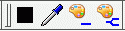
\includegraphics[width=3cm]{images/color-buttons.png}
        \end{center}    
\end{itemize}
El primer bot\'on (de color negro en la imagen de arriba) muestra en color actual. Haciendo click sobre el, le permitir\'a escoger otro color. Tambi\'en puede escoger otro color seleccionando la rama con el color deseado y utilizando el bot\'on de configurar color. Los botones que muestran unas paletas de color, colorean la rama seleccionada con el color actual. Mientras que la primera colorea el encabezado de la selecci\'on, la otra tambi\'en colorea los hijos de la rama seleccionada.

%tipp
Una funci\'on \'util es la de "copiar el color" utilizando el rat\'on: Seleccione la rama que desea colorear, luego presione \key{Ctrl} y simult\'aneamente haga click izquierdo con el rat\'on sobre otra rama para copiar el color a la primera. Los hijos de esa rama tambi\'en obtendr\'ian el nuevo color, si solo desea colorear lo seleccionado adicionalmente presione \key{Shift}.

\subsubsection*{Uso de Banderas}
\vym provee varias banderas. Las puede ver en la parte superior de de la ventana del Editor de mapas. (Nota: Como todas las barras de herramientas puede, moverla hacia el lado izquierdo o derecho e incluso extraerla. Solo agarre la parte punteada a la izquierda de la barra de herramientas con el bot\'on izquierdo del rat\'on.)
\begin{center}
    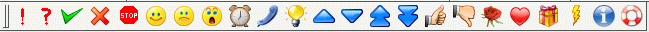
\includegraphics[width=8cm]{images/default-flags.png}
\end{center}
Si tiene una rama seleccionada, puede colocar cualquier numero de banderas con solo hacer click sobre ellas en la barra de herramientas. Los botones en la barra cambian su estado y siempre reflejan el conjunto de banderas en la rama seleccionada.

Actualmente \vym utiliza 2 tipos de banderas: {\em Banderas del Sistema} y {\em Banderas Comunes}. Las bandera comunes son aquellas que aparecen en la barra de herramientas. Las banderas del sistemas son configuradas por el \vym para indicar por ejemplo que hay informaci\'on adicional en una nota (mas acerca de esto en \ref{noteeditor}). Las ultimas versiones de \vym puede que tengan otros tipos de banderas, que pueden ser editadas por el usuario.


\subsubsection*{Im\'agenes}
La forma mas f\'acil de agregar una imagen a una rama es arrastr\'andola, por ejemplo desde un navegador al Editor de mapas mientras la rama se encuentra seleccionada.

Tambi\'en puede agregar una imagen a una rama utilizando el men\'u desplegable, seleccione la opci\'on Adicionar \ra Agregar Imagen. Una ventana de di\'alogo le permitir\'a escoger la imagen que se va a cargar\footnote{Tipo de im\'agenes soportadas: PNG, BMP, XBM, XPM y PNM. Puede que tambi\'en soporte JPEG, MNG y GIF, si es configurado durante la compilaci\'on (como se hace cuando \vym es parte de SUSE LINUX).}.
Mientras seleccione una imagen en la ventana de di\'alogo, podr\'a tener una vista previa de ella. Tambi\'en es posible seleccionar m\'ultiples im\'agenes.

Puede posicionar la imagen donde quiera, solo arrastrela con el bot\'on izquierdo del rat\'on. Para vincularla a otra rama, presione \key{Shift} mientras la mueve. Para borrarla presione \key{Del}.   

Si hace click con el bot\'on derecho sobre una imagen, un men\'u desplegable se abrir\'a el cual le permitir\'a escoger una de varios formatos para im\'agenes. Luego se abrir\'a una ventana de di\'alogo para guardar la imagen. Pista: Esto es utilizado para "exportar" la imagen, de todas formas sera guardado en el mismo mapa!. Tambi\'en pude cortar y copiar la imagen, pero no es posible agregar objetos a una imagen\footnote{
    Las im\'agenes son consideradas como "caracter\'isticas especiales". Trabajar con el mapa seria mas complejo si por ejemplo las im\'agenes estuvieran vinculadas a otras.}
    
La opci\'on \lq{\bf Exportar} \rq controla la salida de exportaciones por ejemplo a HTML: Si esta no esta configurada, la imagen no aparecer\'a en la parte del {\em texto} de salida. Esto es \'util cuando se manejan grandes im\'agenes o im\'agenes utilizadas como bordes, por ejemplo el famoso s\'imbolo en forma de nube en alguna parte del mapa. Esos no deben aparecer en medio del texto.

Por los momentos el soporte de im\'agenes es preliminar: Las im\'agenes ser\'an guardadas junto al resto de la informaci\'on del mapa en el archivo {\tt .vym}.
Versiones futuras incluir\'an mayor funcionalidad como redimensionar el tama\~no, cambiar los valores z (colocarla en el fondo), etc.

\subsubsection*{Bordes}
Un borde puede sera agregado a una rama haciendo click con el bot\'on derecho del rat\'on. Un men\'u desplegable aparecer\'a, en donde podr\'a seleccionarlo. Por el momento solo puede escoger entre un rect\'angulo y "Sin Borde", sin embargo puede utilizar im\'agenes como bordes. De un vistazo al mapa de demostraci\'on {\tt todo.vym}, donde el centro del mapa es una nube. Puede utilizar un programa de dibujo como el {\tt gimp} para crear im\'agenes, preferiblemente con un canal de transparencia, de esta forma podr\'a dise\~nar bordes que no utilizan lineas rectangulares, como la nube.

\subsection{Dise\~no del Fondo}
El dise\~no del fondo del mapa y los links que conectan a distintas partes del mapa pueden ser modificados:

\begin{itemize}
    \item Seleccionando la opci\'on Formato desde el men\'u.
    \item Haciendo click derecho en el espacio entre las ramas, lo cual abrir\'a un men\'u desplegable.
\end{itemize}

\subsubsection*{Color de Fondo}
El color es configurado (y adem\'as mostrado) en Configurar color de fondo.

\subsubsection*{Color del Link}
Los links que conectan  a las ramas tambi\'en pueden ser coloreados en cualquiera de las siguientes formas:
\begin{itemize}
    \item Utilice el color del encabezado donde se encuentra la rama
    \item Utilice {\em un} color para todos los links. El color por defecto es azul.
\end{itemize}
El ultimo puede ser configurado con Set Link Color. Seleccione o no la opci\'on "Usar color para encabezado de enlace" para escoger uno de los 2 dise\~nos para su mapa.

\subsubsection*{Estilo del Link}
\vym Ofrece cuatro estilos diferentes para la apariencia de los links:
\begin{itemize}
    \item Linea
    \item Par\'abola
    \item Linea Gruesa
    \item Par\'abola Gruesa
    
\end{itemize}
Los estilos "grueso" solo se aplican a los links que comienzan en el centro del mapa, el resto del mapa sera dibujado normal.


\subsection{Enlaces hacia otros documentos y p\'aginas web}
\vym soporta dos tipos de enlaces:
\begin{itemize}
    \item Documentos, los cuales se abrir\'an en un navegador externo
    \item Mapa \vym, que se abrir\'a en el mismo \vym.
\end{itemize}
Adicionalmente a los enlaces externos tambi\'en hay enlaces internos, que lo llevan de una rama a otra en el mapa. Esos son llamados {\em XLinks} y son explicados en la secci\'on ~\ref{xlinks}..

\subsubsection*{Webbrowser}
Navegadores modernos como el {\tt konqueror} pueden mostrar distintos tipos de archivos, tanto locales como de la internet. Para introducir la URL de cualquier documento, haga click derecho sobre la rama y seleccione "Editar URL". Introduzca la direcci\'on del documento (o copie y pegue desde el navegador). Los siguientes son ejemplos de direcciones validas:
\begin{verbatim}
    http://www.insilmaril.de/vym/index.html
    file:/usr/share/doc/packages/vym/doc/vym.pdf
\end{verbatim}
Si se ha introducido una URL, un peque\~no globo aparecer\'a en la rama. Haciendo click en el globo que esta en la barra de herramientas o en el men\'u desplegable, un navegador \footnote{
    El navegador puede ser cambiado en el men\'u de configuraci\'on.}
externo se iniciara.
\begin{center}
    
\includegraphics[width=0.5cm]{images/flag-url.png}
\end{center}
Para m\'as informaci\'on sobre el trabajo con marcadores y navegadores web observe la secci\'on \ref{bookmarks}.


\subsubsection*{Mapa \vym}
Para hacer un enlace a otro mapa haga click derecho sobre la rama y seleccione "Edit \ra Enter \vym Link". Una ventana de di\'alogo se abrir\'a donde puede escoger el mapa. Una rama con un enlace es se\~nalada con
\begin{center}
    \includegraphics[width=0.5cm]{images/flag-vymlink.png}
\end{center}
Haciendo click a esta bandera en la barra de herramientas  o en el men\'u desplegable de la rama, abrir\'a el mapa en otra pesta\~na (vea la secci\'on \ref{tabs} para trabajar con m\'ultiples mapas). Para borrar un enlace, solo presione el bot\'on "Cancelar".

Nota: Internamente \vym trabaja con direcciones absolutas para evitar abrir varias ventanas que contengan el mismo mapa. Cuando se guarda un mapa, la direcci\'on se convierte a una relativa (por ejemplo{\tt /home/user/vym.map} se convertir\'ia en {\tt ./vym.map}). Esto facilita el uso de m\'ultiples mapas en distintas computadoras o para exportarlos a HTML en un futuro.

\subsection{M\'ultiples mapas} \label{tabs}
Puede trabajar en varios mapas al mismo tiempo. Cada mapa nuevo es abierto en una nueva {\em pesta\~na}. Las pesta\~nas disponibles se encuentran en la parte superior del editor de mapas. Puede utilizar las funciones de /cortar/copiar/pegar para copiar la informaci\'on de un mapa a otro.

\section{Editor de notas} \label {noteeditor}
Si desea guardar mas texto en una rama como un correo electr\'onico completo, una receta de cocina o todo el c\'odigo fuente de un software, puede utilizar el editor de notas.
\begin{center}
    \includegraphics[width=8cm]{images/noteeditor_es.png}
\end{center}
Este editor muestra el texto asociado a una rama seleccionada en el editor de mapas. Para visualizar que a lo mejor no hay texto todav\'ia, el editor de notas  muestra diferentes colores de fondo dependiendo de su estado:

\subsection{Estados}
Antes de que pueda escribir o pegar texto en el, tiene que seleccionar una rama en el editor de mapas.  F\'ijese que el color de fondo indica el estado del editor:
\begin{itemize}
    \item negro: no ha seleccionado ninguna rama
    \item gris: no ha introducido texto
    \item blanco: el texto esta disponible
\end{itemize}   
Para ver en el editor de mapas si una rama posee una nota con mas informaci\'on, una bandera aparecer\'a junto al encabezado de la rama. Observe la rama en la parte de abajo al lado derecho:
\begin{center}
    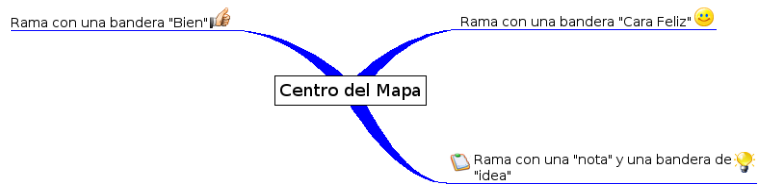
\includegraphics[width=8cm]{images/branches-flags_es.png}
\end{center}

\subsection{Importar y exportar notas}
Las notas siempre son autom\'aticamente guardadas dentro de los archivos  de \vym. Sin embargo, a veces es bueno importarlas desde un archivo externo o escribirlas. Utilice "Archivo \ra Importar" y "Archivo \ra Exportar".

\subsection{Editar e imprimir una nota}
Editar se realiza de la misma forma que en cualquier editor de texto sencillo, incluyendo las funciones rehacer y deshacer. Puede borrar una nota completa haciendo click en la papelera. Solo se imprime la nota si hace click en el icono de la impresora.

Cuando utiliza los mecanismos de copiar\&pegar del X11, el editor creara un p\'arrafo para cada linea nueva. Por lo general esto no se quiere, as\'i que puede convertir todos los p\'arrafos en una sola linea usando la funci\'on "Editar~\ra~Convertir P\'arrafos" o \key{ALT-X}..

\subsection{RichText: Colores, p\'arrafos y texto con formato}
\vym Soporta texto con formato (QT Rich Text) en el editor de notas desde la versi\'on 1.4.7. Colores y atributos del texto (por ejemplo cursiva, negrita) pueden ser seleccionados con los botones que se encuentran arriba del texto. El mismo texto es divido en p\'arrafos. Para cada p\'arrafo se puede configurar un formato (por ejemplo centrado, a la derecha). Un p\'arrafo finaliza cuando \key{Return} es introducido. Si simplemente desea comenzar una nueva linea, presione \key{CTRL-Return}.

\subsection{Fuentes y como cambiarlas r\'apidamente}
El editor de notas esta destinado para ser usado con notas simples y no como un editor de texto con todas las opciones. Debido a la cantidad de peticiones, ahora \vym soporta texto con formato en el editor de notas\footnote{
    \\vym utiliza el formato QRichText, el cual es un subconjunto del formato provisto en HTML.}. 
Dos fuentes por defectos son soportadas las cuales se pueden seleccionar en el men\'u de configuraci\'on. Una es una fuente de ancho definido y la otra es de ancho variable. La fuente de ancho definido es usualmente utilizada en correos electr\'onicos, c\'odigo fuente, etc. Mientras que la fuente de ancho variable es utilizada para notas sencillas, donde no se necesitan caracteres con el ancho definido. Se pueden cambiar las fuentes f\'acilmente utilizando el siguiente s\'imbolo en la barra de herramientas:
\begin{center}
    \includegraphics[width=0.5cm]{images/formatfixedfont.png}
\end{center}
En el men\'u de configuraci\'on ambas fuentes se pueden seleccionar e incluso establecer por defecto.

Adicionalmente a las fuentes por defecto, cualquier fuente instalada en el sistema tambi\'en se podr\'a utilizar. Note que la fuente escogida tambi\'en sera utilizada para las exportaciones en HTML, por lo que deber\'ia usar solo fuentes que se encuentran disponibles generalmente.

\subsection{B\'usqueda de texto}
El editor de notas como tal no posee una funci\'on de b\'usqueda, utilice la que se encuentra en el editor de mapas, que adem\'as busca entre todas las notas (vea la secci\'on \ref{findwindow}).

\subsection{Pegar texto en el editor de notas}
En ocasiones pegara texto en el editor desde otra aplicaci\'on, por ejemplo un correo electr\'onico. Normalmente \vym generara un p\'arrafo por cada linea nueva. Por lo general esto es algo que usted no desea, por lo que puede escoger en el men\'u.

\subsection{Acciones avanzadas}
\subsubsection*{Editar \ra Convertir P\'arrafos:}
Esto convierte texto seleccionado (o todo el texto sino selecciono algo) en lineas consecutivas. Esto es especialmente \'util cuando se trabaja con c\'odigo fuente.


\subsubsection*{Editar \ra Unir L\'ineas:}
Intenta dar formato al texto, de manera que las lineas vac\'ias sean utilizadas para limitar los p\'arrafos del texto seleccionado (o todo sino selecciono algo). Esta funci\'on es \'util para textos como correos electr\'onicos, res\'umenes de reuniones, etc.

\section{Hola Mundo}
Esta secci\'on muestra como \vym interact\'ua con otras aplicaciones. Otras aplicaciones pueden leer y escribir la informaci\'on utilizando XML (eXtensible Markup Language). \vym tambi\'en utiliza XML para guardar los mapas, vea la secci\'on \ref{fileformat}  para una descripci\'on mas detallada.

As\'i que si su aplicaci\'on comprende XML, los dem\'as podr\'an escribir filtros para importar/exportar en \vym. Los voluntarios son siempre bienvenidos


\subsection{Importar} \label{import}

\subsubsection*{Marcadores KDE}
El editor de marcadores integrado en KDE se encuentra de alguna forma limitado, as\'i que ¿porque no utilizar \vym para ordenar los marcadores? Para crear un mapa que contenga los marcadores en KDE seleccione
\begin{itemize}
    \item Archivo \ra Importar\ra KDE Bookmarks
\end{itemize}

\subsubsection*{Mind Manager}
Actualmente \vym cuenta con un filtro b\'asico para convertir mapas creados por {\em Mind Manager}\footnote{
Mind Manager es un software profesional de Mindjet. Ambos nombres son marcas registradas por Mindjet. Para mas informaci\'on visite su p\'agina web: \href{http://mindjet.de}{http://mindjet.de}} dentro de mapas \vym. Las notas e im\'agenes no son convertidas por los momentos. Puede importar archivos con

\begin{itemize}
    \item Archivo \ra Exportar \ra Open Office
\end{itemize}


\subsubsection*{Estructura del Directorio}
\vym puede leer la estructura de un directorio. Esto es principalmente para probar \vym, por ejemplo puede crear f\'acilmente grandes mapas para realizar comparaciones (si, todav\'ia se puede optimizar \vym). ;-)


\subsection{Exportar}  \label{export}
\label{hideexport}
Algunas veces no querr\'a exportar todo el mapa, sino solo una parte de el. Por ejemplo, puede tener informaci\'on adicional la cual mencionara en la presentaci\'on, esas partes no deben estar visibles a la audiencia. Para lograr esto puede "esconder" partes del mapa durante la exportaci\'on seleccionando la bandera de "esconder durante la exportaci\'on"
\begin{center}
    \includegraphics[width=0.5cm]{images/flag-hideexport.png}
\end{center}
Puede escoger esta bandera desde la barra de herramientas o presionando \key{H}. F\'ijese que existe una opci\'on global para el uso de esta bandera en el men\'u de configuraciones. Por defecto se encuentra habilitada.

\subsubsection*{Open Office}
Desde la versi\'on 2 se utiliza el formato de documento de Open Oficce, el cual puede ser escrito por \vym. Las opciones se encuentran limitadas, pero es posible exportar presentaciones que pueden ser abiertas en Open Office Impress. Seleccionando
\begin{itemize}
    \item Archivo \ra  Exportar \ra Open Office
\end{itemize}
Se abrir\'a una ventana de di\'alogo donde podr\'a escoger la salida y el tipo de archivo:
\begin{center}
    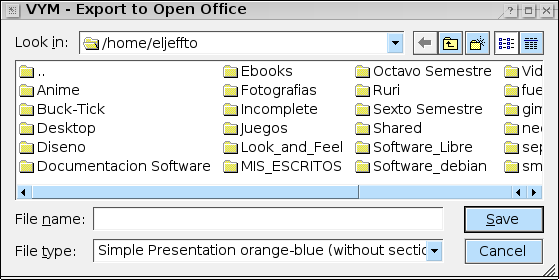
\includegraphics[width=12cm]{images/export-oo_es.png}
\end{center}

El tipo de archivo representa varias plantillas, las cuales se pueden crear con algo de trabajo a mano desde un documento existente en Open Office. Luego se inserta la estructura del mapa \vym en la plantilla. Existen algunas limitaciones por los momentos:
\begin{itemize}
    \item \vym no puede hacerse cargo del largo de las p\'agina, para evitar que el texto se corra mas all\'a del final de la p\'agina tendr\'a que revisarlo y probablemente editarlo en Open Office.
    \item Las im\'agenes y banderas no se utilizan por los momentos
    \item Las notas son escritas en textos simples sin RichText.
\end{itemize}
Algunas de las plantillas hacen uso de {\em secciones} por ejemplo inserta los encabezados de las ramas principales como cap\'itulos para secciones dentro de una presentaci\'on.
Some of the templates make use of {\em sections} e.g. insert the
headings of mainbranches as chapters for sections into the presentation.

\subsubsection*{Imagen}
\vym soportar todos los formatos de imagen que son originalmente soportadas por las herramientas de QT: BMP, JPEG, PBM, PGM, PNG, PPN, XPN y XBM. Para utilizar en sitios web y enviar im\'agenes por correo electr\'onico se recomienda PNG, el cual considera la calidad y el tama\~no de la imagen. \vym utiliza las opciones de QT por defecto para comprimir las im\'agenes.

\subsubsection*{ASCII}
    Exportar una imagen como texto es algo experimental hasta los momentos. Probablemente se podr\'a hacer luego con el uso de hojas de estilo. As\'i que el resultado puede cambiar en futuras versiones de \vym.

\subsubsection*{\LaTeX}
\vym puede generar un archivo de entrada para \LaTeX. Esto es considerado como experimental, todav\'ia no existen opciones. Seleccionado
\begin{itemize}
    \item   Archivo \ra Exportar \ra \LaTeX
\end{itemize}
    se le preguntara en una ventana de di\'alogo por el nombre del archivo de salida. Este archivo debe ser incluido en el documento \LaTeX utilizando el comando
\begin{verbatim}
    \include{inputfile.tex}
\end{verbatim}

\subsubsection*{Marcadores KDE}
\vym sobreescribir\'a el archivo de marcadores de KDE e intentar\'a notificar a los konquerors el cambio del archivo v\'ia DCOP. 
¡ \vym no crea copias de seguridad !
\begin{itemize}
    \item Archivo \ra Exportar \ra KDE Bookmarks
\end{itemize}

\subsubsection*{XHTML (Paginas Web)}

Este es el formato que querr\'as utilizar para crear una p\'agina web. Por ejemplo observa la p\'agina oficial de \vym:
\href{http://www.InSilmaril.de/vym}{www.InSilmaril.de/vym}

Una explicaci\'on de como trabaja esto: 
Antes de que un mapa es exportado a XHTML, sera escrito primero como XML en un directorio (ver \ref{xmlexport}). Luego el programa externo {\tt
xsltproc} \footnote{En Linux SUSE xsltproc es instalado por defecto.}  
sera llamado para procesar el archivo XML y genera el c\'odigo HTML. Una ventana de di\'alogo le permite escoger varias opciones:
\begin{itemize}
    \item {\bf Incluir una imagen:}  Si esta configurado, \vym creara un mapa de imagen en la parte superior de la salida HTML. Haciendo click sobre una rama del mapa lo llevara a la secci\'on correspondiente de la salida.
    \item {\bf Encabezados con color:}
    Si esta seleccionado, \vym coloreara los encabezados en el texto con los mismos colores del mapa.
    \item {\bf Mostrar Advertencias: }
    Si esta seleccionado, \vym preguntara primero antes de sobreescribir la informaci\'on,
    \item {\bf Mostrar la salida:}
    Esto resulta \'util principalmente para la depuraci\'on. Mostrara como el procesamiento del archivo XML trabaja, llamando a  {\tt xsltproc}.
\end{itemize}
Adem\'as las direcciones para el CSS y XSL stylesheets se pueden configurar. Por defecto en LINUX SUSE se encuentran en
{\tt /usr/share/vym/styles}.


 varios mapas combinados tienen que ser guardados en el mismo directorio.
\subsubsection*{XML} \label{xmlexport}

El mapa es escrito dentro de los directorios como una imagen y como XML. El directorio se selecciona en una ventana de di\'alogo. Si el directorio no esta vac\'io, se le preguntara si se arriesga a sobreescribir su contenido.

Es posible exportar diferentes mapas a un mismo directorio. Cada archivo generado tendr\'a el nombre del mapa como un prefijo, por ejemplo {\tt todo.vym} se convertir\'a en {\tt todo.xml}, {\tt todo.png}, {\tt todo-image-1.png} y as\'i sucesivamente. Esto es \'util si por ejemplo para una p\'agina web.

\subsubsection*{Exportar una parte del mapa}
Seleccione la rama que desea exportar junto a sus hijos, luego en el men\'u desplegable y seleccione {\em Guardar Selecci\'on}. Esto creara un archivo con la extensi\'on {\tt .vyp}, el cual es la abreviaci\'on de \lq \vym part\rq.

\section{Edici\'on Avanzada}

\subsection{Como trabajar con Marcadores} \label{bookmarks}
\subsubsection*{Abra una nueva pesta\~na en vez de una nueva ventana}
Si usa konqueror como buscador, \vym recordar\'a el konqueror que fue abierto antes por \vym. Tambi\'en puede presionar \key{Ctrl} y de click para abrir el link en una nueva pesta\~na.

\vym tambi\'en puede abrir pesta\~nas en Mozilla o Firefox usando el comando remoto\footnote{\href{http://www.mozilla.org/unix/remote.html}{http://www.mozilla.org/unix/remote.html}}
para estos.

\subsubsection*{Arrastrar y soltar}
Si desea mantener el marcador en el mapa, seleccione una rama donde deseee agregar el marcador,
despu\'es simplemente arrastre la URL desde su buscador hasta el mapa. Tambi\'en puede usar un encabezado existente como 
URL: Click derecho sobre la rama y selecciones "Usar encabezado por URL".

\subsubsection*{Acceso directo a la lista de marcadores de un buscador}
Por favor observe las secciones \ref{import} y \ref{export} about
Import and Export filters.

\subsubsection*{URLs especiales}
\vym puede tornar un encabezado existente de una rama en una URL. Actualmente
este trabaja para ingreso de Bgus en un sistema de Bugtracking de Novell: Abra el 
men\'u de contexto de una rama (usualmente click derecho en \'el) y seleccione
\begin{itemize}
    \item Crear URL con Bugzilla
\end{itemize}
La URL ser\'a constuida desde el n\'umero en la cabecera.

\subsection{Incluir im\'agenes en uan rama} 
La configuraci\'on por defecto de una im\'agen flotar "libremente". Estas pueden ser
posicionadas en cualquier lugar, pero siempre terminar\'an en el mismo lugar como
las otras partes del mapa.

La soluci\'on es incluirla "dentro" de uan rama. Esto puede ser hecho v\'ia
el men\'u de contexto de su rama padre:
\begin{itemize}
    \item Incluir imagen horizontalmente
    \item Incluir imagen verticalmente
\end{itemize}
La imagen a\'un no est\'a posicionada relativa a su rama padre, pero el
encabezado y borde de la rama se adaptan a la im\'agen flotante, observe a continuaci\'on:
\begin{center}
    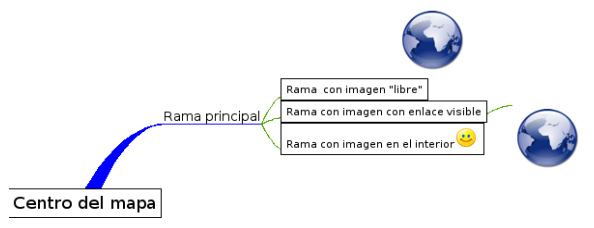
\includegraphics[width=11cm]{images/includeImages_es.png}
\end{center}

\subsection{Modificadores} 
Los modificadores son por ejemplo las teclas \key{Shift} o \key{Alt}. Mientras se presionan junto con el rat\'on, estos ocasionan que \vym utilice las acciones "modificadas". Por ejemplo puede mover las ramas con el rat\'on. Si presiona \key{Ctrl} o \key{Alt} mientras suelta la rama, esta sera agregada por encima o debajo del blanco pero no como un hijo.

Sin un modificador presionado, el primer click a una rama solo la selecciona. Para crear el comportamiento de \key{Ctrl} hay varias opciones, que pueden ser seleccionadas desde la barra de herramientas:


\begin{center}
    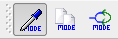
\includegraphics[width=3cm]{images/modmodes.png}
\end{center}
Por defecto esta copiar el color de la rama donde hicimos click a la que seleccionaremos. En la barra de herramientas el modificador por defecto esta seleccionado para copiar el color de la rama.  El segundo modificador le permite f\'acilmente copiar el color de una rama entera con un solo click. El tercer modificador le permite crear {\em xLinks}, los cuales se explicaran en la siguientes secci\'on.

\subsection{Esconder enlaces de objetos no seleccionados}
A veces es \'util posicionar libremente una rama, como una rama principal o una imagen. Aunque esto no es posible (todav\'ia) para todas las ramas, puede utilizar una rama y ocultar su enlace de conexi\'on al centro del mapa. Se pude utilizar por ejemplo con leyendas o una colecci\'on de Links de \vym que apuntan a otros mapas:

\begin{center}
    \includegraphics[width=9cm]{images/hiddenlink_es.png}
\end{center}


\subsection{XLinks} \label{xlinks}
Hasta ahora todo la informaci\'on en el mapa \vym se parece a la de un \'arbol. Utilizando xLinks puede enlazar una rama con otra, como amarrando una cuerda entre las dos ramas en un \'arbol real. Esto es muy \'util en mapas complejos, donde se quiera tener referencias cruzadas que no se ajusten al \'area visible en la pantalla. El siguiente ejemplo, el cual forma parte del paquete \vym, se ajusta a la pantalla, pero muestra como la informaci\'on puede estar entrelazada. En el gr\'afico hay un enlace desde una tarea (prepara una presentaci\'on) hacia informaci\'on general:

\begin{center}
    \includegraphics[width=12cm]{images/xlink_es.png}
\end{center}
F\'ijese que un xLink que apunta a una rama que no se encuentra visible (porque estas acoplada), se muestra como una peque\~na flecha horizontal. En la imagen de la pantalla arriba observe la rama \lq Jueves\rq\ .

\subsubsection*{Crear un xLink}
Seleccione el tipo de link en el modificador de la barra de herramientas (haciendo click o presionando \key{L}. Seleccione la rama donde el xLink comenzara. Presiones la tecla modificadora \key{Ctrl} y simult\'aneamente haga click sobre la rama donde el enlace terminara. (El enlace es dibujado antes de que suelte el bot\'on del rat\'on). Si suelta el rat\'on sobre una rama el xLink se volver\'a permanente.

\subsubsection*{Modificar o borrar un xLink}
En el men\'u desplegable de la rama seleccione la opci\'on \lq Editar xLink\rq. Un submen\'u contiene todos los xLinks de la rama (si existe alguno). Son nombrados como las ramas donde finalizan. Seleccione uno y se abrir\'a una ventana de di\'alogo, donde puede seleccionar el color, ancho o borrar el xLink.

\subsubsection*{Seguir un xLink}
En un mapa complejo \vym resulta \'util saltar al final del xLink. Puede realizar esto a trav\'es del men\'u desplegable de la rama y haciendo click en \lq Ir a xLink\rq y seleccione el xLink que desea seguir.

\subsection{Agregando y removiendo ramas}
El men\'u desplegable de una rama muestra mas formas de agregar y borrar informaci\'on por ejemplo puede borrar una rama y conservar sus hijos.  Los hijos se enlazan al padre de la rama que fue removida. Ramas parecidas pueden insertarse a mapas existentes. Para atajos en el teclado revise el men\'u desplegable.

\subsection{Agregando un mapa o parte de el}
Seleccione la rama donde desea agregar un mapa guardado ({\tt .vym}) o parte de un mapa ({\tt .vyp}), luego en el men\'u desplegable seleccione {\em Agregar \ra Importar}. Para importar puede escoger ente {\em Agregar o Reemplazar}: La informaci\'on importada se agregar\'a o reemplazar\'a la selecci\'on.

\section{\vym en Mac OS X}
\subsection{Descripci\'on}
B\'asicamente existen 2 maneras para correr \vym en Macs:
\subsubsection*{Edici\'on QT Mac:}
    \vym esta disponible como una aplicaci\'on comprimida para Mac OS X. Ha sido compilada u probada en Mac OS 10.3, Pero tambi\'en debe trabajar en Tiger. Utilizando la versi\'on Mac de la librer\'ia Trolltechs QT. 
\subsubsection*{X11}
    \vym puede tambi\'en correr la versi\'on de Linux, pero entonces los men\'us y el manejo tambi\'en ser\'an como los de esa versi\'on de Linux, por ejemplo la barra del men\'u se vera diferente. 

\subsection {Men\'u desplegable y teclas especiales}

La mayor\'ia de las Mac desafortunadamente tienen un solo bot\'on para el rat\'on. Para mostrar el men\'u desplegable, el cual se abre con el bot\'on derecho del rat\'on, puede hacer click mientras presiona una tecla \key{kommand}.

Especialmente en port\'atiles faltan algunas de las teclas utilizadas en los ordenadores de escritorio. La edici\'on QT-Mac de \vym tiene sus propios atajos por teclado. Para conseguir los atajos solo eche un vistazo a todas las funciones del men\'u, junto observara los atajos. Los botones de la barra de herramientas tambi\'en poseen atajos, solo coloque el puntero del rat\'on sobre el bot\'on y espere a que aparezca la peque\~na ventan de ayuda.

\subsection {Visualizando enlaces externos}

En Mac, \vym usa la llamada al sistema {\tt /usr/bin/open} para ver los enlaces. Mac OS determina autom\'aticamente si el enlaces es un 

\begin{appendix}

\section{Iniciando \vym}
\subsection{Direcci\'on para recursos}
\vym intentara encontrar sus recursos (im\'agenes, hojas de estilo, filtros, etc.) en las siguientes ubicaciones:
\begin{enumerate}
    \item Direcci\'on dada por la variable del entorno {\tt VYMHOME}.
    \item 1.Si fue llamado por una opci\'on local (vea la secci\'on \ref{options} m\'as adelante), \vym buscara por la informaci\'on en el 
    \item {\tt /usr/share/vym}
    \item {\tt /usr/local/share/vym}
\end{enumerate}

\subsection{Opciones de la linea de comando.} \label{options}
\vym tiene las siguientes opciones
\begin{center}
\begin{tabular}{ccp{8cm}}\\ 
\bf Opci\'on    & \bf Comentario & \bf Descripci\'on \\ \hline
v & versi\'on & Muestra la versi\'on de \vym \vym\\
l & local   & Utiliza direcciones locales para hojas de estilo, traducciones, iconos, etc. \'Util para realizar pruebas\\
h & ayuda   & Muestra ayuda\\
q & abandonar   & Abandona inmediatamente luego de haber iniciado. \'Util para realizar comparaciones.\\
\end{tabular}
\end{center}
Tambi\'en puede dar varios nombres de archivo en la linea de comando para que \vym abra varios mapas al mismo tiempo.
 
\section{Contribuyendo con \vym}
Hasta ahora he dicho que he escrito 98\% del c\'odigo yo mismo. No es sorpresa que \vym se adapte a mis necesidades. Sin embargo me gustar\'ia animar a todos los usuarios de \vym a contribuir. No solo con peticiones para mejorar opciones, sino tambi\'en con el c\'odigo, nuevos filtros para importar/exportar, traducciones, etc. En este ap\'endice tratare de mostrar lo f\'acil que es expandir las cosas que puede actualmente hacer con \vym. Espero pronto saber de ustedes!

\subsection{Obteniendo ayuda}

\subsubsection*{Preguntas t\'ipicas (FAQ)}
Dir\'ijase a FAQ disponible en la p\'agina web de \vym:
\begin{center}
\href{http://www.InSilmaril.de/vym/faq.html}{http://www.InSilmaril.de/vym/faq.html}
\end{center}

\subsubsection*{Listas de correo}
Existen dos listas de correo: {\tt vym-forum} es el foro de los usuarios de \vym para discutir las preguntas, mientras que {\tt vym-devel} esta dirigida a gente que desea contribuir con \vym. Puede revisar los archivos y suscribirse en
\begin{center}
\href{https://sourceforge.net/mail/?group_id=127802}{https://sourceforge.net/mail/?group\_id=127802}
\end{center}

\subsubsection*{Contactar al autor}\label{author}
Intente en la listas de correo primero si necesita soporte t\'ecnico. Si todo lo anterior falla puede contactar al Uwe Drechsel a
\begin{center}
\href{mailto:vym@InSilmaril.de}{vym@InSilmaril.de}
\end{center}

\subsubsection*{Contactar los traductores}\label{author}
Para indicar errores de traducci\'on, sugerencias y afines envie un correo a
\begin{center}
\href{mailto:aclibre@gmail.com}{aclibre@gmail.com}
\end{center}



\subsection{Como reportar errores}
A pesar de que Sourceforge tiene su propio sistema para reportar errores, preferir\'ia que me contactara primero (vea la secci\'on \ref{author}) e incluso mejor: Puede reportar el error en Bugzilla, el sistema de reporte de errores del sistema de openSUSE:
\begin{center}
\href{http://en.opensuse.org/Submit_a_bug}{http://en.opensuse.org/Submit\_a\_bug}
\end{center}
Yo compilo \vym regularmente para openSUSE, as\'i que deber\'ia reportarlo all\'i aunque utilice otro Sistema Operativo. No olvide mencionar
\begin{itemize}
    \item Los pasos exactos necesarios para reproducir el error
    \item La versi\'on y fecha del \vym (vea Ayuda \ra Acerca de \vym)
    \vym)
    \item Hardware y Sistema Operativo
\end{itemize}

\subsection{Compilando desde el C\'odigo Fuente}
\subsubsection{Obteniendo las fuentes} \label{getsources}
Encontrara la ultima versi\'on de \vym en el sitio del proyecto:
\begin{center}
\href{https://sourceforge.net/projects/vym/}{https://sourceforge.net/projects/vym/}
\end{center}
All\'i puede ver los repositorios (CVS) del c\'odigo fuente:

\begin{verbatim}
cvs -d:pserver:anonymous@cvs.sf.net:/cvsroot/vym checkout code
\end{verbatim}

\subsubsection{Herramientas Qt}
Qt es un conjunto de herramientas de C++ para el desarrollo de aplicaciones e interfaces gr\'aficas multiplataforma. Provee de un solo c\'odigo portable entre MS Windows, Mac OS X, Linux y todas las variantes comerciales de Unix. Qt tambi\'en esta disponible para dispositivos integrados. Qt es un producto Trolltech. Para mas informaci\'on:
\begin{center}
\href{http://www.trolltech.com/qt/}{www.trolltech.com/qt} 
\end{center}


\subsubsection{Compilando \vym}
Aseg\'urese de que instalo el entorno Qt apropiadamente, vea la documentaci\'on de Qt para mas detalles. Necesita tener el comando {\tt qmake} en las variables de entorno, luego ejecute

\begin{verbatim}
qmake
make  
make install
\end{verbatim}
El ultimo comando make install necesita los permisos de root. Por su puesto se puede omitir, si solo desea probar \vym.

%\subsubsection*{Compiling \vym on Macs}
%TODO

\subsection{Formato de los archivos \vym } \label{fileformat}
Por lo general los mapas tienen la extensi\'on "{\tt .vym}" y representan un archivo comprimido de la informaci\'on. Si desea tener una vista a fondo de la estructura de la informaci\'on del mapa llamado "mapname.\vym", descomprima el mapa manualmente utilizando
\begin{verbatim}
    unzip mapname.vym
\end{verbatim}
Esto creara directorios llamados {\tt images} y {\tt flags} en el directorio actual y en el propio mapa, por lo general llamado mapname.xml. La estructura XML de \vym se explica por si sola, solo eche un vistazo a {\tt mapname.xml}.

El archivo XML puede ser cargado directamente en \vym, no tiene que estar comprimido. Si desea comprimir toda la informaci\'on utilice
\begin{verbatim}
    zip -r mapname.vym .
\end{verbatim}
para comprimir la informaci\'on del directorio donde se encuentra.

\subsection{Nuevas Opciones}
Existen muchas opciones que han encontrara en \vym. Junto con \vym recibi\'o un directorio con algunos mapas, por ejemplo en SUSE LINUX 
\begin{center}
    {\tt /usr/share/doc/packages/vym/demos}
\end{center}
donde encontrara el mapa {\tt todo.vym}. Muestra muchas cosas que se har\'an en el futuro. Si tiene mas ideas, conecte al equipo desarrollador a 
{\tt vym-devel@lists.sourceforge.net}.


\subsection{Soporte a nuevos lenguajes}
Para agregar otro lenguaje a \vym necesita el c\'odigo fuente (vea la secci\'on \ref{getsources})  y la instalaci\'on de Trolltechs QT. Una parte de QT son las herramientas de desarrollo, de esas herramientas es necesaria la herramientas de traducci\'on "Lingü\'istica".

En algunas distribuciones de Linux las herramientas de desarrollo se encuentran en un paquete extra, por ejemplo en SUSE LINUX debe instalar:
\begin{verbatim}
    qt3-devel.rpm
    qt3-devel-doc.rpm
    qt3-devel-tools.rpm
    qt3-man.rpm
\end{verbatim}
Sino posee QT en su sistema, lo puede conseguir en 
    \href{http://www.trolltech.com}{http://www.trolltech.com}
Una vez que ya pueda compilar \vym, puede traducir el texto de \vym realizando los siguientes pasos:
\begin{itemize}
    \item Supongamos que la codificaci\'on es "Nueva" en lugar de "de" para el alem\'an o "es" para el espa\~nol
    
    \item Copie el archivo {\tt lang/vym\_en.ts} en {\tt ang/vym\_Nueva.ts} (El propio c\'odigo contiene la versi\'on en ingles). 
        
    \item Agregue  {\tt lang/vym\_Nueva.ts} a la secci\'on de TRADUCCIONES de \vym.pro. 

    \item Ejecute Linguist en {\tt vym\_Nueva.ts} y realice la traducci\'on.  

    \item Ejecute {\tt lrelease}  para crear {\tt vym\_Nueva.qm} to create 

    \item Ejecute make install para instalar el nuevo \vym y revisar la traducci\'on.
\end{itemize}

Si lo desea tambi\'en puede traducir el manual. Esta escrito en LaTeX, solo debe cambiar el archivo text/\vym.tex. (Linguist o QT no se necesitan pero si se necesita saber como trabajar con LaTeX, espec\'ificamente pdfltex para crear un PDF).

Por favor env\'ie todas las traducciones que realice. Tambi\'en puedo darle acceso como desarrollador en el proyecto, si desea proveer traducciones regularmente.

\subsection{Nuevos filtros para exportar e importar}
\vym soporta distintos tipos de filtros. La informaci\'on puede ser escrita directamente, insertada en plantillas o escrita como XML y luego procesada por transformaciones XSL.

Muchas de las funciones de importar/exportar se encuentra en las clases ImportBase y ExportBase y subclases. Estas las pueden conseguir en {\tt imports.h} y {\tt exports.h}.

\subsubsection*{Importa y Exportar directamente}
n ejemplo de exportaci\'on directa es el de XML. Este m\'etodo toca las implementaciones de casi todos los objetos de \vym, as\'i que mientras pueda mejor utilice transformaci\'on XSL.

Si todav\'ia quiere saber como se realiza esto, comience por observar
{\tt MapEditor::saveToDir} en {\tt mapeditor.cpp}.

\subsubsection*{Plantillas}
Las plantillas se introducen para exportar a formatos opendoc utilizados por ejemplo por Open Office. Mientras leo las especificaciones (menor a 500 paginas) acerca del formato\footnote{
\href{http://www.oasis-open.org/}{http://www.oasis-open.org/}}\ 
me da la sensaci\'on de que no quiero escribir la exportaci\'on desde el inicio. Seria muy complejo adaptar el estilo a sus propios deseos, por ejemplo el layout.

En su lugar analizo los documentos existentes del Open Office. Encontr\'e que existen un gran numero de bits redundantes en la informaci\'on de una presentaci\'on cl\'asica, por ejemplo cada lista de detalles es contenida en su propia lista. Al final expuse el estilo de la presentaci\'on por defecto, que todav\'ia puede ser simplificado, solo en caso de que tenga tiempo libre\ldots

Las plantillas existentes todav\'ia est\'an bajo desarrollo, antes de que pase mucho tiempo desarrollando su propio estilo, por favor contacteme. B\'asicamente se necesitan los siguientes pasos para construir su propio estilo:
\begin{enumerate}
    \item Crea un ejemplo en Open Office. Utilice un titulo, nombre de autor, encabezado de pagina, etc. \ que f\'acilmente puede escoger para la salida del archivo.
    
    \item Descomprima el documento Open Office en un directorio.

    \item El archivo principal es llamado {\tt content.xml}. Toda la informaci\'on esta en una sola linea. Puede dividir las etiquetas XML utilizando el script {\tt    scripts/niceXML}, el cual es parte de la distribuci\'on de \vym.

    \item Copie la salida de  {\tt niceXML} en {\tt content-template.xml}.

    \item Observe que encontrara un gran numero de definiciones sin utilizar, por ejemplo de algunos estilos. Los puede borrar o simplemente ignorarlos.

    \item 1.Intente encontrar su titulo, nombre de autor. \vym reemplazara las siguientes cadenas mientras realiza la exportaci\'on:
    \begin{center}
    \begin{tabular}{lp{4cm}}
        {\tt <!-- INSERT TITLE -->}     & title of map \\
        {\tt <!-- INSERT AUTHOR-->  }   & author \\
        {\tt <!-- INSERT COMMENT -->}   & comment \\
        {\tt <!-- INSERT PAGES-->}      & content of map \\
    \end{tabular}
    \end{center}
    El contenido es generado de manera similar insertando listas en {\tt page-template}. Se realizan las siguientes sustituciones:
    \begin{center}
    \begin{tabular}{lp{7cm}}
        {\tt <!-- INSERT PAGE HEADING-->}       & Encabezado de la pagina (rama principal o                                     hijo de la rama principal, dependiendo                          del uso de las secciones). \\
        {\tt <!-- INSERT LIST -->   }   & Todos los hijos de ramas de arriba. \\
    \end{tabular}
    \end{center}
\end{enumerate}
Actualmente las im\'agenes son exportadas y las notas solo aparecen como texto sin formato y colores.


\subsubsection*{Transformaciones XSL}
\vym utiliza transformaciones XSL mientras exporta (por ejemplo XHTML) e importa informaci\'on (por ejemplo marcadores KDE). Se necesita de un poco de c\'odigo para la interfaz gr\'afica del usuario, el resto es realizado utilizando la hoja de estilo {\tt .xsl} e invocando el procesador {\tt xsltproc}, el cual forma parte de libxslt, la librer\'ia XSLT C para GNOME.

\end{appendix}
\end{document}
\end{document}

